\documentclass[12pt]{article}

\title{Lab Assignment 4}
\author{Cameron Mattson}

% import a set of useful packages for math
\usepackage{amsmath, amsfonts, amssymb}
\usepackage{tcolorbox}
\usepackage{multirow}

% this package makes margins smaller
\usepackage{fullpage}
\usepackage{listings}
\usepackage{amsmath}
\usepackage{graphicx}
\usepackage{listing}
% for importing images
%%%%%%%%%%%%%%%%%%%%%%%%%%%%%%%%
\begin{document}
\maketitle
\tableofcontents
\section{Code}
\begin{lstlisting}[breaklines=true]
img_dir = "https://vizwiz.cs.colorado.edu//VizWiz_visualization_img/"

# Read the file to extract each dataset example with label
import requests
import numpy as np
from skimage import io
from keras.layers import TextVectorization
import numpy as np
import tensorflow as tf
import cv2
from collections import Counter
from tensorflow.keras.utils import to_categorical

splits = ['train', 'val', 'test']
data_splits = []
embed_dim = 100
vectorizer = TextVectorization(max_tokens=20600, output_sequence_length=embed_dim)

# Splitting the data into different sets eg. (train, validation, test)
for split in splits:
    annotation_file = "https://ivc.ischool.utexas.edu/VizWiz_final/vqa_data/Annotations/%s.json" %split
    split_data = requests.get(annotation_file, allow_redirects=True)
    data_splits.append(split_data.json())

# Extract Vocab from validation and training splits
train_questions = [s['question'] for s in data_splits[0]]
question_pool = train_questions

text_ds = tf.data.Dataset.from_tensor_slices(question_pool).batch(128) ## Read batches of 128 samples
vectorizer.adapt(text_ds)
vocab = vectorizer.get_vocabulary()

train_samps = 2000
val_samps = 500
test_samps = 1000
num_classes = 1000

y_train_ques = []
y_val_ques = []
y_test_ques = []
y_train_ques_samp = []
y_val_ques_samp = []
y_test_ques_samp = []

# Create embedding matrix for train data
X_train_ques = vectorizer(np.array([[s['question']] for s in data_splits[0][:train_samps]]))

for samp in data_splits[0][:train_samps]:
  # retrieve the first answer from each question image pair for truth labels
  y_train_ques.append(samp['answers'][0]['answer'])

  # Build the list of all possible answers from the train set to create the most frequent answers
  for ans_list in samp['answers']:
    y_train_ques_samp.append(ans_list['answer'].lower())

for samp in data_splits[1][:val_samps]:
   # retrieve the first answer from each question image pair for truth labels
  y_val_ques.append(samp['answers'][0]['answer'])
  
  # Build the list of all possible answers from the validation set to create the most frequent answers
  for ans_list in samp['answers']:
    y_val_ques_samp.append(ans_list['answer'].lower())

# Find the 1000 most frequent answers
ans_counter = Counter(y_val_ques + y_train_ques_samp)
most_freq = ans_counter.most_common(num_classes)
y_ques = np.array([ans[0] for ans in most_freq])
y_ques_enc = to_categorical(np.arange(num_classes))
ind_default = np.nonzero(y_ques == 'unanswerable')[0]
if (ind_default.shape[0] < 1):
  ind_default = num_classes-1
  y_ques[ind_default] = 'unanswerable'
else:
  ind_default = ind_default[0]

y_train_ind = []

# Use the most frequent answers to assign labels to each answer in the training set
for ans in y_train_ques:
  match = False

  for ind, freq_ans in enumerate(y_ques):
    if (freq_ans == ans):
      match = True
      y_train_ind.append(ind)
      break
  # If the training example is not found, assign it the 'unnasigned' label at index 0
  if (not match):
    y_train_ind.append(ind_default)

y_val_ind = []
# Use the most frequent answers to assign labels to each answer in the training set
for ans in y_val_ques:
  match = False

  for ind, freq_ans in enumerate(y_ques):
    if (freq_ans == ans):
      match = True
      y_val_ind.append(ind)
      break

  # If the training example is not found, assign it the 'unnasigned' label at index 0
  if (not match):
    y_val_ind.append(ind_default)

y_train_ind_enc = np.zeros((train_samps, num_classes))
y_train_ind_enc[np.arange(len(y_train_ind)),y_train_ind] = 1
y_train_ind_enc.astype(np.int64)

y_val_ind_enc = np.zeros((val_samps, num_classes))
y_val_ind_enc[np.arange(len(y_val_ind)),y_val_ind] = 1
y_val_ind_enc.astype(np.int64)

X_val_ques = vectorizer(np.array([[s['question']] for s in data_splits[1][:val_samps]]))
X_test_ques = vectorizer(np.array([[s['question']] for s in data_splits[2][:test_samps]]))
X_train_img = np.array([cv2.resize(io.imread(img_dir + s['image']), (360, 480)) for s in data_splits[0][:train_samps]])
X_val_img = np.array([cv2.resize(io.imread(img_dir + s['image']), (360, 480)) for s in data_splits[1][:val_samps]])
X_test_img = np.array([cv2.resize(io.imread(img_dir + s['image']), (360, 480)) for s in data_splits[2][:test_samps]])

from keras.models import Sequential, Model
from keras.layers import LSTM, Conv2D, MaxPooling2D, Dense, Input, Flatten, Concatenate, Embedding, Dropout
tf.keras.utils.set_random_seed(24)

def vqa_mod1(): # Higher LSTM and convolutional emphasis
  inputs_cnn = Input(shape=(480, 360, 3))
  inputs = Conv2D(15, (3, 3), activation='relu', padding='same', input_shape=(480, 360, 3))(inputs_cnn)
  inputs = MaxPooling2D((2, 2))(inputs)
  inputs = Conv2D(15, (3, 3), activation='relu', padding='same', input_shape=(480, 360, 3))(inputs)
  inputs = MaxPooling2D((2, 2))(inputs)
  inputs = Conv2D(15, (3, 3), activation='relu', padding='same', input_shape=(480, 360, 3))(inputs)
  inputs = MaxPooling2D((2, 2))(inputs)
  inputs = Flatten()(inputs)

  question_input = Input(shape=(None,), dtype="int64")
  embedded_sequences = Embedding(len(vocab), embed_dim, trainable=True)(question_input)
  lstm_mod = LSTM(256, return_sequences=True)(embedded_sequences)
  lstm_mod = LSTM(256)(lstm_mod) # Recently added

  merged = Concatenate()([inputs, lstm_mod])
  output = Dense(num_classes, activation='softmax')(merged)
  mymod = Model([inputs_cnn, question_input], output)

  mymod.compile(loss = 'categorical_crossentropy', optimizer = 'adam', metrics = 'accuracy')
  #mymod.summary()

  mymod.fit([X_train_img, X_train_ques], y_train_ind_enc, batch_size=100, epochs=15, verbose=0, shuffle=True)

  return mymod

def vqa_mod2(): # Higher LSTM and convolutional emphasis
  inputs_cnn = Input(shape=(480, 360, 3))
  inputs = Conv2D(15, (3, 3), activation='relu', padding='same', input_shape=(480, 360, 3))(inputs_cnn)
  inputs = MaxPooling2D((7, 7))(inputs)
  inputs = Flatten()(inputs)

  question_input = Input(shape=(None,), dtype="int64")
  embedded_sequences = Embedding(len(vocab), embed_dim, trainable=True)(question_input)
  lstm_mod = LSTM(256, return_sequences=True)(embedded_sequences)
  lstm_mod = LSTM(256)(lstm_mod) # Recently added

  merged = Concatenate()([inputs, lstm_mod])
  output = Dense(num_classes, activation='softmax')(merged)
  mymod = Model([inputs_cnn, question_input], output)

  mymod.compile(loss = 'categorical_crossentropy', optimizer = 'adam', metrics = 'accuracy')
  #mymod.summary()

  mymod.fit([X_train_img, X_train_ques], y_train_ind_enc, batch_size=100, epochs=15, verbose=0, shuffle=True)

  return mymod

def vqa_mod3(): # Higher LSTM and convolutional emphasis
  inputs_cnn = Input(shape=(480, 360, 3))
  inputs = Conv2D(15, (3, 3), activation='relu', padding='same', input_shape=(480, 360, 3))(inputs_cnn)
  inputs = MaxPooling2D((2, 2))(inputs)
  inputs = Conv2D(15, (3, 3), activation='relu', padding='same', input_shape=(480, 360, 3))(inputs)
  inputs = MaxPooling2D((2, 2))(inputs)
  inputs = Conv2D(15, (3, 3), activation='relu', padding='same', input_shape=(480, 360, 3))(inputs)
  inputs = MaxPooling2D((2, 2))(inputs)
  inputs = Flatten()(inputs)

  question_input = Input(shape=(None,), dtype="int64")
  embedded_sequences = Embedding(len(vocab), embed_dim, trainable=True)(question_input)
  lstm_mod = LSTM(256)(embedded_sequences) # Recently addedb

  merged = Concatenate()([inputs, lstm_mod])
  output = Dense(num_classes, activation='softmax')(merged)
  mymod = Model([inputs_cnn, question_input], output)

  mymod.compile(loss = 'categorical_crossentropy', optimizer = 'adam', metrics = 'accuracy')
  #mymod.summary()

  mymod.fit([X_train_img, X_train_ques], y_train_ind_enc, batch_size=100, epochs=15, verbose=0, shuffle=True)

  return mymod

# Use np.argmax of the ground-truth labels to see if there are any matches
def comp_acc(mypreds, cdataset):
  acc = []
  for pred_ind, pred in enumerate(mypreds):
    pred_labels = []
    word_pred = y_ques[pred]
    for samp in data_splits[cdataset][pred_ind]['answers']:
    # retrieve the first answer from each question image pair for truth labels
      #print(data_splits[1][pred_ind])
      pred_labels.append(samp['answer'])
    num_match = np.nonzero(word_pred == np.array(pred_labels))[0].shape[0] # Find matching labels to compute the accuracy
    acc.append(min((num_match / 3), 1))
    # Calculate the number of matches and from there calculate the 'special' accuracy metric
  return acc

import gc

mymod1 = vqa_mod1()
mypreds1 = mymod1.predict([X_val_img, X_val_ques])
myacc1 = comp_acc(np.argmax(mypreds1, axis=1), 1)
del mymod1
del mypreds1
gc.collect()

mymod2 = vqa_mod2()
mypreds2 = mymod2.predict([X_val_img, X_val_ques])
myacc2 = comp_acc(np.argmax(mypreds2, axis=1), 1)
del mymod2
del mypreds2
gc.collect()

mymod3 = vqa_mod3()
mypreds3 = mymod3.predict([X_val_img, X_val_ques])
myacc3 = comp_acc(np.argmax(mypreds3, axis=1), 1)

print(f'Mean Accuracy on model 1 = {round(np.mean(myacc1),2)}')
print(f'Mean Accuracy on model 1 = {round(np.mean(myacc2),2)}')
print(f'Mean Accuracy on model 1 = {round(np.mean(myacc3),2)}')

import pandas as pd
mypreds4 = mymod3.predict([X_test_img, X_test_ques])
mypreds4 = y_ques[np.argmax(mypreds4, axis=1)]
df = pd.DataFrame(mypreds4)
df.to_csv("results.csv", header = None, index = None)
del mymod3
del mypreds3
gc.collect()

def vqa_mod4(myepochs): # Higher LSTM and convolutional emphasis
  inputs_cnn = Input(shape=(480, 360, 3))
  inputs = Conv2D(15, (3, 3), activation='relu', padding='same', input_shape=(480, 360, 3))(inputs_cnn)
  inputs = MaxPooling2D((2, 2))(inputs)
  inputs = Conv2D(15, (3, 3), activation='relu', padding='same', input_shape=(480, 360, 3))(inputs)
  inputs = MaxPooling2D((2, 2))(inputs)
  inputs = Conv2D(15, (3, 3), activation='relu', padding='same', input_shape=(480, 360, 3))(inputs)
  inputs = MaxPooling2D((2, 2))(inputs)
  inputs = Flatten()(inputs)

  question_input = Input(shape=(None,), dtype="int64")
  embedded_sequences = Embedding(len(vocab), embed_dim, trainable=True)(question_input)
  lstm_mod = LSTM(256)(embedded_sequences) # Recently addedb

  merged = Concatenate()([inputs, lstm_mod])
  output = Dense(num_classes, activation='softmax')(merged)
  mymod = Model([inputs_cnn, question_input], output)

  mymod.compile(loss = 'categorical_crossentropy', optimizer = 'adam', metrics = 'accuracy')
  #mymod.summary()

  mymod.fit([X_train_img, X_train_ques], y_train_ind_enc, batch_size=100, epochs=myepochs, verbose=0, shuffle=True)

  return mymod

train_acc = []
val_acc = []
i = 0
for epoch in range(1,16):
  i += 1
  print(epoch)
  mymod1 = vqa_mod4(epoch)
  mypreds1 = mymod1.predict([X_train_img, X_train_ques])
  train_acc.append(round(np.mean(comp_acc(np.argmax(mypreds1, axis=1), 0)),2))
  mypreds2 = mymod1.predict([X_val_img, X_val_ques])
  val_acc.append(round(np.mean(comp_acc(np.argmax(mypreds2, axis=1), 1)),2))
  del mymod1
  del mypreds1
  del mypreds2
  gc.collect()

import matplotlib.pyplot as plt
epochs = np.arange(1,16)
plt.plot(epochs, train_acc, color = 'green', label = 'Training')
plt.plot(epochs, val_acc, color = 'orange', label = 'Validation')
plt.xlabel('Epoch')
plt.ylabel('Accuracy')
plt.title('VQA Model Performance')
plt.legend()
plt.savefig('vqa_model.png')
plt.show()
\end{lstlisting}
\newpage
\section{Write-up}
\subsection{Methods}
In this experiment three models were created. Each model concatenated the outputs of two constituent models similar to the baseline model used in the Visual Question Answering (VQA) task. These constituents were the LSTM model and the CNN model. Each model was designed to vary the number of weights and layers in each of these constituents to evaluate relative contributions. The first model consisted of the maximum number of weights and layers of any constituent model designed in this experiment. Specifically, the LSTM constituent model contained two LSTM layers and the CNN model contained three convolutional layers and 3 max pooling layers. The second model used fewer weights and layers in the CNN constituent model than the first model, and the same number weights and layers in the LSTM constituent model as in the first model. The last max pooling layer in the second model's constituent CNN model had a 7 by 7 pooling size, which was larger than the pooling sizes used in any of the other models. In the third model, the model architecture was the same as with the first model, except the constituent LSTM model was designed with one less LSTM layer.\\
\\
In every model described above the CNN constituent model consisted of 3 convolutional layers which alternated with max pooling layers. Each of these convolutional layers had 15 maps, and used a three by three kernel, same padding, and relu activation functions. Likewise, all pooling layers used in each of these models were max pooling layers of size two by two, with the exception of the max pooling layer in model two described above. Each LSTM layers consisted of 256 units with all other parameters being set to the default values. Similarly, the convolutional layers and max pooling layer parameters were set by default unless stated.\\
\\
The LSTM constituent models used in this experiment took inputs sequences of size 100 for each word, whereas the CNN constituent models took resized images as inputs of size 480 by 360 by 3. Once these models were concatenated, the softmax was computed using the predefined 1000 classes, and the models were compiled using categorical cross entropy, the adam optimizer, and the accuracy metric. Then the models were fit using a batch size of 100 and 15 epochs.\\
\\
Each of these models were created to predict the answer from 1000 of the most popular answer choices using the training and validation sets. Not all of the answer choices availble were sufficient for every sample. Therefore, an 'unanswerable' option was included in the 1000 most popular answers to handle these cases. The design relied on creating a word embedding of the questions in the training set, and using a randomly choosen answer for each sample in the training set to update weights and biases of each model. To train each model, the GPU in google collab was utilized in this experiment.\\
\\
In the second part of this experiment, the third model was choosen to predict the results of the test set. This model was exclusively trained on the traing data with all of the same hyperparameters as the third model in the previous part of this experiment. This model was also used to evaluate the performance on the visual question answering task using both the training set and the validation set.\\
\\
To complete this assignment, code from the coding tutorials was incorporated as well as information from the professor's lectures.
\subsection{Results}
\begin{table}[h!]
\caption{Model Accuracy on Validation Set}
\centering
\begin{tabular}{||c c||} 
 \hline
 Model & VQA Accuracy \\ [0.5ex] 
 \hline\hline
 Model 1 (Control) & 0.38 \\ 
 Model 2 (Smaller CNN Constituent)& 0.36 \\
 Model 3 (Smaller LSTM Constituent) & 0.42 \\ [1ex]
 \hline
\end{tabular}
\end{table}

\begin{center}
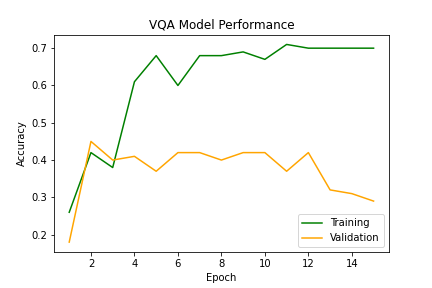
\includegraphics[scale=1]{vqa_model.png}
\end{center}
\newpage
\subsection{Analysis}
For each of the models trained in this experiment the VQA accuracy was relatively the same, with the second model having the lowest VQA accuracy, and the third model having the highest VQA accuracy. These accuracies are shown in Table 1 above. From these results we can see that the top performing models had larger CNN constituent models with more layers and weights. When the constituent models are concatenated, the CNN model has tens of thousands of outputs, whereas the LSTM has 256 outputs. Therefore we may expect the CNN constituent model to determine the predicted output more accurately than the LSTM constituent model in each of the models evaluated. Another trend that we observe is that the third model with the smaller LSTM constituent model performs the best, whereas the model with with larger LSTM constituent models perform worse. This may due to overfitting, since the LSTM constituent model in the third model is less complex than the other LSTM constituent models designed in this experiment. Similarly, since all of the VQA accuracies are relatively close in value, this could also be the result of chance. \\
\\
The third model performed better on the training data than on the validation data when trying to answer questions using images as shown in the plot above. The performance of the model on the training set increased at first and then started to converge, while the performance of the model on the validation set remained relatively constant and then started to decrease after epoch 12. In thise case the model was overfitting, and the model didn't seem to perform better after epoch two. A likely explanation could be due to the way that the model was predicting the output. Since the model was only considering the 1000 most common answers, if most of the outputs were unanswerable than the model may overgeneralize when predicting the outputs. As a result, the model may perform poorly, and yet learn quickly to overgeneralize within a few epochs. However, if a model that combined the inputs more naturally such as LXMERT was used, I think we would observe substatially better results.
\end{document}